\section{Introduction}

    \subparagraph{}Le but de ce {\color{info}8\ieme{} travail} travail est de mettre en oeuvre des D flip-flop à partir
     de la fonction logique du travail précédent, générer un registre de 4 bits sous la forme d'un sous-circuit, 
     concevoir un sous-circuit de la fonction logique à 4 entrée et vérifier son fonctionnement correct en parcourant 
     la table de vérité avec la fréquence de la table de vérité fisxé à 500 MHz puis jusqu'a la valeur maximale 
     garatissant encore son bon fonctionnement. Enfin, il faudra comparer cette valeur avec le temps de propagation du
      travail précédent et pour finir de 
    simuler le circuit avec le logiciel \textit{LTspice} afin de démontrer l'exactitude des calculs.\\[1.5cm]
    
    \begin{titletbox}{À l'attention du correcteur / correctrice}{warning}
        N'hésitez pas à zoomer sur les schémas du circuit et autres images afin d'y voir plus clair.
    \end{titletbox}

    \section{Rappel de la fonction logique}

    \subsection{Table de vérité}
    
        \subparagraph{}Au travail précédent, j'avais construit la table de vérité de ma fonction Y :
        
            \begin{table}[H]
                \centering
                \begin{tabular}{|c|c|c|c|
                >{\columncolor[HTML]{DAE8FC}}c |}
                \hline
                \textbf{A} & \textbf{B} & \textbf{C} & \textbf{D} & \textbf{Y}                                       \\ \hline
                0          & 0          & 0          & 0          & 1                                                \\ \hline
                0          & 0          & 0          & 1          & 0                                                \\ \hline
                0          & 0          & 1          & 0          & \cellcolor[HTML]{CB0000}X                        \\ \hline
                0          & 0          & 1          & 1          & 0                                                \\ \hline
                0          & 1          & 0          & 0          & 0                                                \\ \hline
                0          & 1          & 0          & 1          & \cellcolor[HTML]{CB0000}{\color[HTML]{000000} X} \\ \hline
                0          & 1          & 1          & 0          & 1                                                \\ \hline
                0          & 1          & 1          & 1          & 1                                                \\ \hline
                1          & 0          & 0          & 0          & 0                                                \\ \hline
                1          & 0          & 0          & 1          & \cellcolor[HTML]{CB0000}X                        \\ \hline
                1          & 0          & 1          & 0          & 1                                                \\ \hline
                1          & 0          & 1          & 1          & \cellcolor[HTML]{CB0000}X                        \\ \hline
                1          & 1          & 0          & 0          & 0                                                \\ \hline
                1          & 1          & 0          & 1          & 1                                                \\ \hline
                1          & 1          & 1          & 0          & 0                                                \\ \hline
                1          & 1          & 1          & 1          & 1                                                \\ \hline
                \end{tabular}
                \caption{Table de vérité de la fonction logique}
                \label{tab:truth}
            \end{table}
    
    \subsection{Diagramme de Karnaugh}
    
        \subparagraph{}De cette table logique, on en déduisait le diagramme de Karnaugh suivant :
        
            \begin{center}
                \begin{karnaugh-map}[4][4][1][][] % note empty X and Y labels
                \maxterms{1,2,3,4,12,11} % où se trouve les 0
                \minterms{0,7,13,15,9,10} % où se trouve les 1
                \autoterms[X] % tous les autres endroits => X
                \implicant{5}{15} % les lots à prendre (le rouge)
                \implicantedge{0}{0}{8}{8} % les lots à prendre si ça implique les bords (le vert)
                \implicantedge{8}{8}{10}{10} % lot à prendre (le jaune)
                \implicant{8}{9} % lot à prendre (le bleu)
                % note: posistion for start of \draw is (0, Y) where Y is
                % the Y size(number of cells high) in this case Y=4
                \draw[color=black, ultra thin] (0, 4) --
                node [pos=0.8, above right, anchor=south west] {\textcolor{red}{$A B$}} % x0 x1 label
                node [pos=0.6, below left, anchor=north east] {\textcolor{red}{$C D$}} % x2 x3 label
                ++(135:1);
              \end{karnaugh-map}
            \end{center}
    
    \subsection{Fonction logique}
    
        \subparagraph{}Grâce au diagramme du travail précédent, on obtenait la fonction suivante : 
        
            \begin{equation*}
                Y\;=\;\color{mygreen}\overline{A}\overline{B}\overline{C} + \color{cyan} \overline{A}C\overline{D} + \color{kred} BD + \color{kyellow}\overline{B}C\overline{D}
             \end{equation*}

\section{Schéma du circuit}

    \begin{figure}[H]
        \centering
        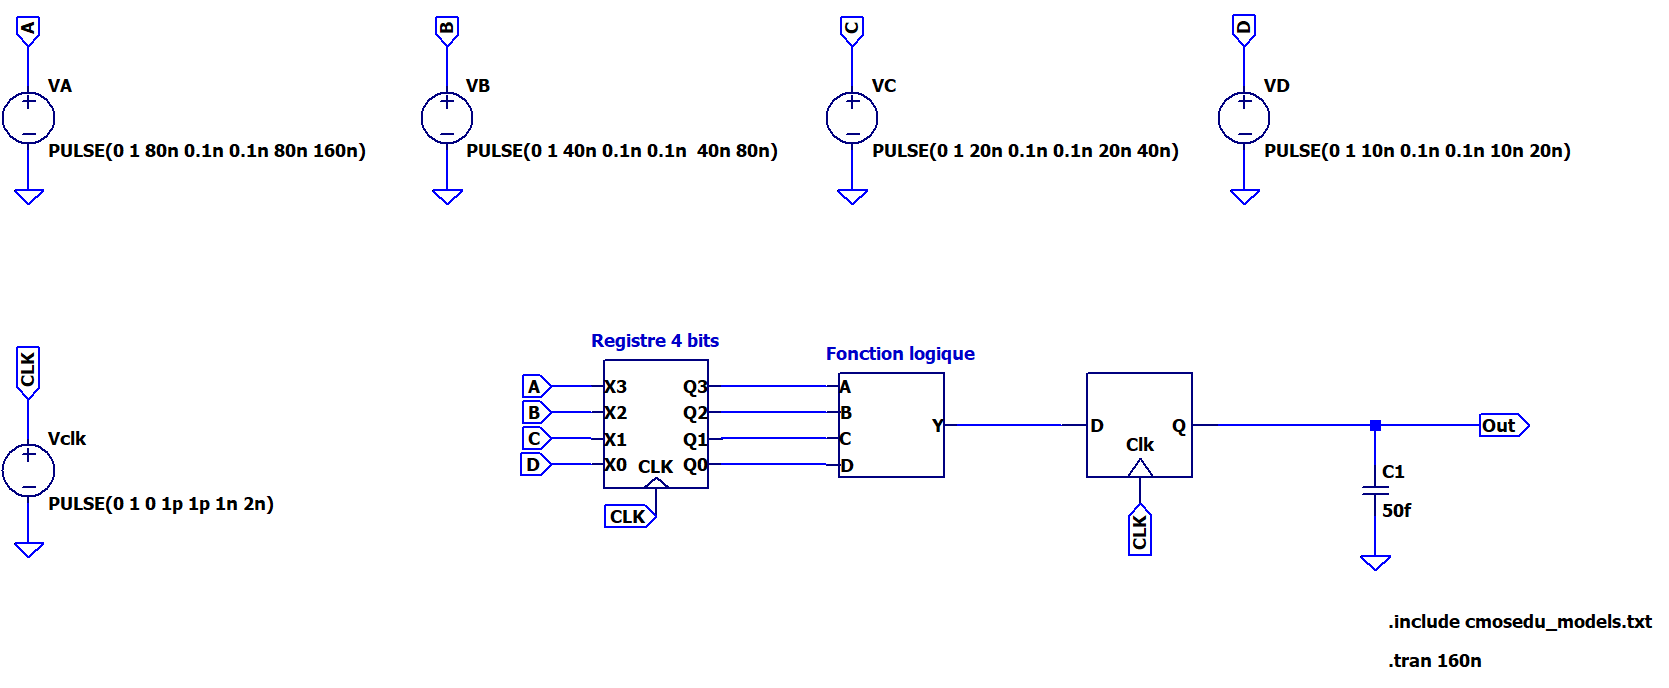
\includegraphics[width=\textwidth]{../pictures/Circuit.PNG}
        \caption{Schéma du circuit}
    \end{figure}
    
    \subparagraph{}Pour $V_A, V_B, V_C, V_D$ il faut reprendre les \textit{PULSE} du travail précédent. Quand à la valeur de la clock, elle doit valoir 500 $MH_Z$. Pour trouver la bonne période pour avoir la bonne \textit{PULSE}, il suffit d'appliquer la formule suivante :
    
        {\color{mygreen}\begin{align*}
            F\;&=\;\frac{1}{T}\;\text{\color{black}(F est la fréquence et T la période)}\\
            T\;&=\;\frac{1}{F}\\
            T\;&=\;\frac{1}{5 \cdot 10^8}\\
            T\;&=\;2\;ns\\
        \end{align*}}
        
        \begin{empheq}[box=\fbox]{equation*}
        \color{red}
            T\;=\;2\;ns
        \end{empheq}

    \subparagraph{}La période est donc de 2 nano-secondes pour avoir une fréquence de 500 $MH_Z$.


\section{Résultat de la simulation en parcourant la table de vérité}

    \begin{figure}[H]
        \centering
        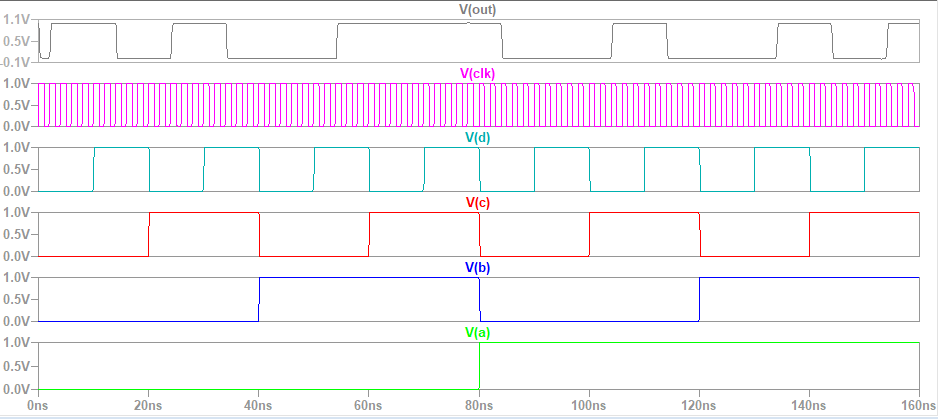
\includegraphics[width=\textwidth]{../pictures/simu-table.PNG}
        \caption{Simulation du circuit à 500 $MH_Z$}
    \end{figure}

    \subparagraph{}On remarque la simulation parcourt et correspond à la table de vérité mais il y a un petit décalage pour les résultats de \textit{out}. Ceci s'explique par le fait que comme les D flip-flop sont à flan montant (rising edge) par rapport à l'horloge et donc que les variations ne sont pas suffisantes pour faire « réagir » les inputs.
    
    
\section{Résultat de la simulation à fréquence maximale}

    \subparagraph{}Pour la fréquence maximale, j'obtiens une clock avec les paramètres suivant :
    
        \begin{figure}[H]
            \centering
            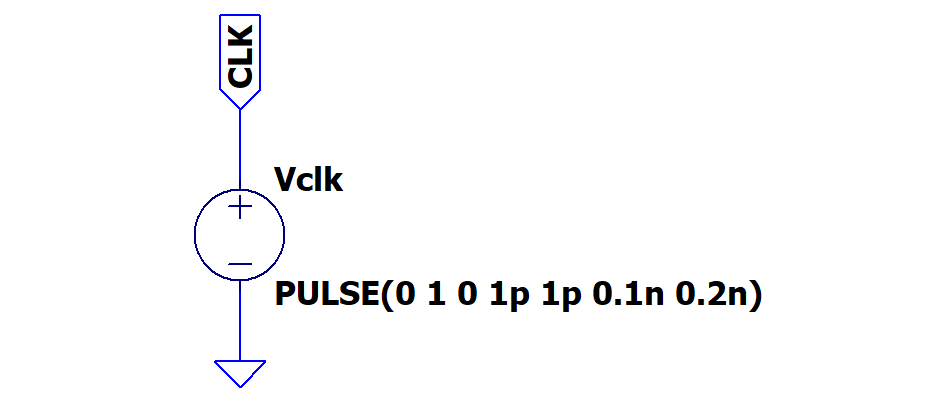
\includegraphics[scale=0.5]{../pictures/Fmax.PNG}
            \caption{Paramètres de la \textit{PULSE} avec la $F_{Max}$}
        \end{figure}
        
        
    \subparagraph{}On a donc la simulation suivante :
    
    \begin{figure}[H]
        \centering
        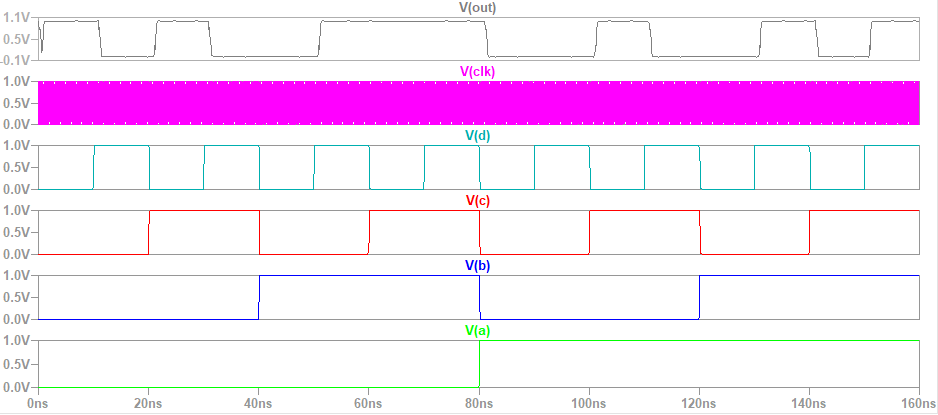
\includegraphics[width=\textwidth]{../pictures/simu-Fmax.PNG}
        \caption{Simulation du circuit à $F_{Max}$}
    \end{figure}
        
    \subparagraph{}On peut calculer la fréquence maximale : 
    
        {\color{mygreen}\begin{align*}
            F_{Max}\;&=\;\frac{1}{T}\;\text{\color{black}(F est la fréquence et T la période)}\\
            F_{Max}\;&=\;\frac{1}{2 \cdot 10^{-10}}\\
            F_{Max}\;&=\;5 \cdot 10^9\;H_Z \\
            F_{Max}\;&=\;5\;GH_Z \\
        \end{align*}}
        
        \begin{empheq}[box=\fbox]{equation*}
        \color{red}
            F_{Max}\;=\;5\;GH_Z
        \end{empheq}
        
        
    \subparagraph{}En mettant la fréquence à 5,26 $GH_Z$ ( \textit{PULSE(0 1 0 1p 1p 0.95n 0.19n)} ) on remarque 
    directement que le résultat n'est plus bon : 
    
        \begin{figure}[H]
        \centering
        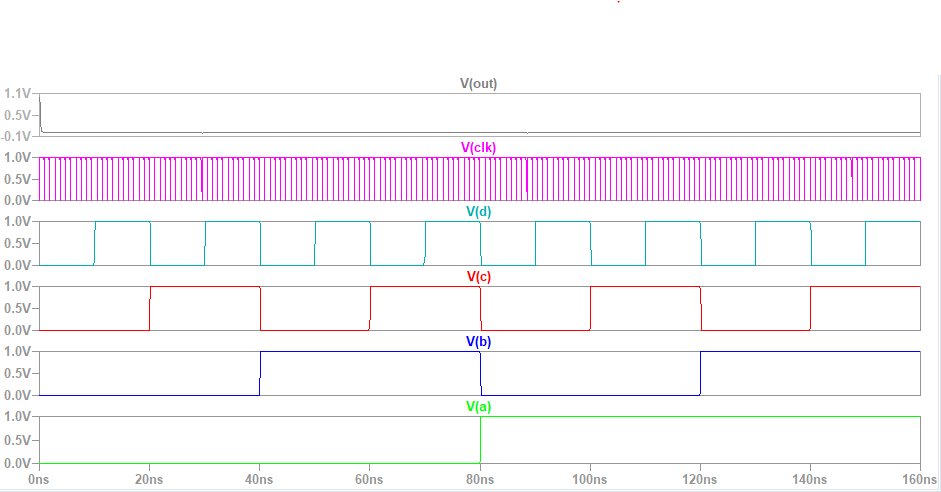
\includegraphics[width=\textwidth]{../pictures/simu-trop.PNG}
        \caption{Simulation du circuit à une fréquence trop élevée}
    \end{figure}

\section{Conclusion}

    \subparagraph{}En premier lieu comparons $F_{max}$ au temps de propagation. Au travail précédent j'avais estimé que 
    le temps de propagation ($t_{pd}$) valait 0.36 nanosecondes. Pour la fréquence maximale ($F_{Max}$), on a une 
    période de 0.2 nanosecondes. On remarquera donc une différence de 1.6 nanoseconde et aussi que la $F_{Max}$ vaut exactement $\frac{5}{9}\;(\approx\;0,556)$ du $t_{pd}$ estimé.
    
    \subparagraph{}Pour conclure, les résultats que j'ai obtenu sont en accord avec la simulation des 16 états de la 
    fonction logique. Ce travail permet de bien appréhender le focntionnement des D flip flop ainsi que des horloges et 
    de mieux comprendre comment fonctionnent les registres.

\end{document}